\documentclass[10pt,twocolumn]{article}

% use the oxycomps style file
\usepackage{oxycomps}

% usage: \fixme[comments describing issue]{text to be fixed}
% define \fixme as not doing anything special
\newcommand{\fixme}[2][]{#2}
% overwrite it so it shows up as red
\renewcommand{\fixme}[2][]{\textcolor{red}{#2}}
% overwrite it again so related text shows as footnotes
%\renewcommand{\fixme}[2][]{\textcolor{red}{#2\footnote{#1}}}

% read references.bib for the bibtex data
\bibliography{references}

% include metadata in the generated pdf file
\pdfinfo{
    /Title (Comps Proposal)
    /Author (Wilson Schwegler)
}

% set the title and author information
\title{Comps Proposal}
\author{Wilson Schwegler}
\affiliation{Occidental College}
\email{schwegler@oxy.edu}

\begin{document}

\maketitle

\section{Introduction}
Traffic sign recognition is a critical aspect of self-driving and intelligent transportation systems. Cars with Advanced Driver Assistance Systems have become very popular and are indicating that self-driving cars are in our future. I have become very interested in this topic and have decided that it will be the basis of my comps topic. The topic for my comps project is to compare the performance of YOLOv8 and Faster R-CNN to my own architecture to determine which is best suited for traffic sign recognition in video.

\section{Problem Context}
Traffic signs play a crucial role in ensuring road safety as they communicate vital information to drivers. They enforce traffic laws, warn of upcoming dangers, guide navigation, and enhance pedestrian safety. Without road signs, there would be chaos and confusion on the roads and an increase in accidents and injuries. While traffic signs increase road safety, it is still dependent on the drivers to obey them. It has been reported that in four US cities, nearly 700,000 police-reported motor vehicle crashes occur annually at stop signs \textcite{NIH}. This means that while stop signs are in place, drivers are still getting in accidents potentially due to missing or not obeying them. 

In order to prevent human error, starting in the 1970s, cars have had Advanced Driver Assistance Systems (ADAS) implemented. The goal of an ADAS system is to help the driver operate the vehicle more safely through early warnings and system automation \textcite{HistoryofADAS}. The National Safety Council has said that ADAS has the potential to largely improve roadway safety and each year, more vehicles are being equipped with these systems \textcite{nsc}. In 2022 the three most implemented ADAS features were rear cameras, rear parking sensors, and front crash prevention \textcite{nsc2}. While these features help reduce the number of accidents caused by distracted driving (the leading cause of accidents in California \textcite{K}), they fail to address accidents caused by distracted driving that involve missed traffic signs. 

Real-time and reliable traffic sign recognition software can improve overall driver safety by reducing accidents caused by missed traffic signs. This research is aimed at understanding if YOLOv8, Faster R-CNN, or a model of my own design is best suite for this task.  

\section{Technical Background}
Object detection algorithms play a crucial role in tasks like traffic sign recognition. This project focuses on comparing three different object detection architectures: YOLOv8, Faster R-CNN, and a model of my own design. All three approaches aim to identify, classify, and label traffic signs within a video frame.

Deep learning is a sub-field of machine learning. It utilizes neural networks which consist of multiple interconnected layers that can learn complex patterns utilizing data \textcite{intel}. Convolutional Neural Networks (CNNs) are a specific type of deep learning architecture that is well-suited for image and video analysis/recognition \textcite{intel}. CNNs are good at extracting features from grid-like data (images) through convolutional layers \textcite{intel}. These layers apply filters to the input data to identify important features like edges, lines, and shapes \textcite{intel}. Pooling layers then reduce the complexity of the data while preserving key information \textcite{intel}. The fully connected layers combine the extracted features to classify and recognize objects within images \textcite{intel}. This approach allows CNNs to perform tasks like object detection and recognition with high accuracy \textcite{intel}. 

\begin{figure}[h]
    \centering
    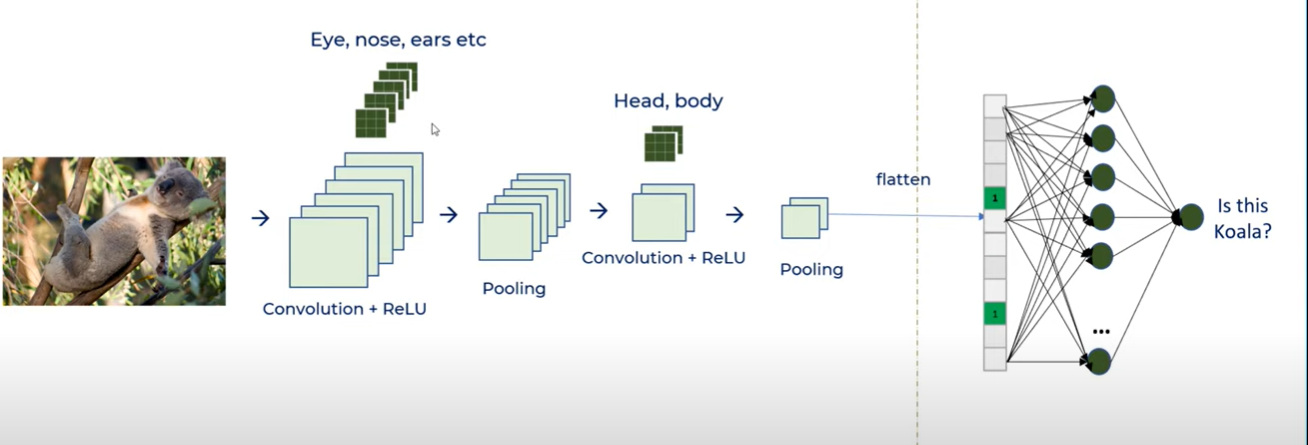
\includegraphics[width=.95\linewidth]{CNN.png}    \caption{
        Simplified Convolutional Neural Network (CNN) architecture for image classification \textcite{LI}
    }
    \label{fig:first-page}
\end{figure}

Figure 1 depicts a simplified CNN for image classification, specifically identifying a koala. The input image on the left side feeds into the convolutional layers. These layers apply filters to extract features like edges and shapes relevant to koalas. Pooling layers then reduce the data complexity. The network includes an additional set of convolutional and pooling layers. This is done so the model can learn more intricate features and be more accurate at image classification. The flattened layer takes the final pooling layer's output and transforms it into a suitable format for the connected layers. The final layer predicts the probability of the image belonging to a specific class. 


You Only Look Once (YOLOv8) is a deep learning model designed for real-time object detection in computer vision applications \textcite{keylabs}. Its ability to detect objects in real-time has major implications for processes like traffic sign recognition. YOLOv8 is a single stage model, meaning that it goes from the image directly to bounding boxes and class probabilities in one shot. This makes YOLOv8 fast and suitable for real-time applications. YOLOv8 requires a Python environment and is built on PyTorch \textcite{keylabs}. PyTorch is a framework for building deep learning models. It is commonly utilized in projects pertaining to image recognition and language processing \textcite{PyTorch}. YOLOv8 allows users to create custom models for their object detection needs. This feature will be utilized in my project by fine-tuning the model on a specific dataset to improve the accuracy and performance of traffic sign recognition \textcite{keylabs}.

Faster R-CNN is a model specializing in object detection. It improves upon Fast R-CNN by implementing a region proposal network (RPN) with the CNN \textcite{R-CNN}. An RPN is a convolutional network that predicts object bounds and objectness scores at each position \textcite{RPN}. The RPN is the first stage of the model. It identifies areas with potential objects. This is done efficiently without going into too much detail. The second stage thoroughly investigates the proposed regions to classify the image. This makes Faster R-CNN a two stage model that can provide accurate results. However due to this, this can make Faster R-CNN slower than other models like YOLOv8.

\section{Prior Work}
There are numerous examples of traffic sign image classification projects available online on websites like Kaggle. However, these projects focus on the implementation of one method and often do not consider alternative designs. My research is aimed at considering two very powerful models and determining if I can create my own model that can perform better at traffic sign recognition in video. The prior work that we will be focusing on is one project from Kaggle and two research papers. The project is a traffic sign detection project using YOLOv8. The first paper is research on traffic sign recognition based on CNN and the second is research on traffic sign classification using faster R-CNN and YOLOv4.  

\subsection{Traffic Signs Detection Using YOLOv8}
This project was conducted by a user on Kaggle by the name of Parisa Karimi Darabi. This project was done in Python and Jupyter Notebook while utilizing a data set that contains traffic and railway signs in Germany \textcite{Darabi}. Darabi first discusses how to implement the pre-trained YOLOv8 model for traffic sign detection. She also discusses what Mean Average Precision (mAP) is, stating that it calculates the precision of each category and averages the scores to determine an overall assessment of the algorithm's performance \textcite{Darabi}. This metric can be used to evaluate the effectiveness of object detection algorithms. It also discusses the steps that should be taken if the mAP obtained is not satisfactory including, extending the training process, experimenting with different parameter values, adjusting the batch size, tuning the initial learning rate, experimenting with different learning rate range values, and selecting a different optimizer \textcite{Darabi}. After tuning the model Darabi concluded that the model had a satisfactory precision of approximately 93 percent \textcite{Darabi}t. Darabi then showed how to implement this trained model with video and yielded satisfactory results \textcite{Darabi}. 

This project is important to my research as it provides an outline of how to implement YOLOv8 as well as how to use it for traffic sign detection in video. It also discusses mAP which is a useful metric that will be utilized in the evaluation of the models that I build. While Darabi provided the tuning that was used to yield her results further testing will be done utilizing the data set for my project in order to determine what adjustments must be made to yield the best results. Projects like this one will be crucial for my own research as having no experience with machine learning they provide a baseline for me to start learning and expand upon in order to answer my research topic. 

\subsection{Relevant Research}
Njayou Youssouf conducted research on traffic sign classification using his own CNN and detection using Faster R-CNN and YOLOv4 \textcite{Youssouf}. Youssouf utilized the German Traffic Sign Data Base for his research. He discusses how he pre-processed the data by addressing the varying image sizes and color variations. He did this by resizing all of the images to a fixed size and converted them to grayscale before feeding them to the CNN for classification \textcite{Youssouf}. Youssouf developed a CNN utilizing Python and TensorFlow. He outlined his lightweight model and discussed implementing Faster R-CNN and YOLOv4. The Faster R-CNN and YOLOv4 models were trained on a smaller data set but showed promising results with minor fine-tuning \textcite{Youssouf}. The model outlined in this paper achieved a high accuracy of 99.20 percent with minimal loss \textcite{Youssouf}. Youssouf justified the model's high accuracy through his pre-processing techniques \textcite{Youssouf}. Similarly, Xiaoxuan Qiao's research discusses the importance of the pre-processing technique utilized \textcite{HSV}. Qiao states that inaccurate segmentation can easily occur during traffic sign detection as R, G, and B components tend to blend in with the background objects when illumination occurs \textcite{HSV}. To solve this, Qiao proposes converting RGB images to HSV (hue, saturation, and lightness). He outlines the process he took to do this as well as outlined his CNN design. Through several iterations of his model, Qiao was able to produce a model with the German Traffic Sign Data Base that had a recognition accuracy of 99.9 percent \textcite{HSV}. 

Both of these research papers provide valuable insight for my project. Youssouf provides a descriptive outline of his CNN's architecture and Qiao discusses his pre-processing process that yielded great results. While Youssouf also tests the same two models, Faster R-CNN and YOLOv4, that my research intends to do, he did not train all of the models on the same data \textcite{Youssouf}. He also did not evaluate all three models on the same evaluation metrics \textcite{Youssouf}. Another glaring difference between his research and my intended research is YOLO has gone through various iterations and is now at version 8 compared to version 4 discussed in his paper. My research will use these two pieces of prior work as a reference to help me build my model's architecture and refine my pre-processing technique. All three pieces of prior work utilized the same data set. I intend to explore a different data set that is composed of traffic signs from the US. 

\section{Methods}
This section will discuss the methods that I intend to utilize for my Senior Comps project. I will first discuss the options for my data set followed by my intended procedure of implementing my own CNN, YOLOv8, and Faster R-CNN. 

\subsection{Data Set}
The most popular data set used for traffic sign recognition projects is the German Traffic Sign Data Base. While this is a well-tested and comprehensive data set, I will not be using it for my project as I want to focus on US traffic signs. Therefore, I will be using a data set from Roboflow called US Road Signs Image Dataset \textcite{dataSet}. This data set consists of a total of 664 images, 468 of them being part of the training set, 98 of them being art of the valid set, and 98 test images \textcite{dataSet}. This data set has had no pre-processing or augmentations done \textcite{dataSet}. This is a relatively small data set compared to the German Traffic Sign Data Base, however it only consists of common US road signs and does not contain traffic lights. The three categories of signs include are regulatory signs, warnings signs, and stop signs. The data set consists of varying lighting and weather conditions as well as different angles \textcite{dataSet}. 

To pre-process the data, the techniques that will be utilized will align with Qiao's research. The images will first be resized to a constant size to address the varying sizes. Then converting the images from RGB to HSV will be done. The calculations to convert  RGB to HSV is shown in Figure 2 \textcite{HSV}. 

\begin{figure}[h]
    \centering
    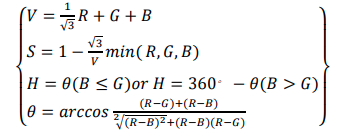
\includegraphics[width=.95\linewidth]{conv.png}    \caption{
        conversion from RGB to HSV \textcite{HSV}
    }
    \label{fig:first-page}
\end{figure}

Based off of Qiao's research, conversion from RGB to HSV will yield better results then just converting the image to gray scale \textcite{HSV}. After completing these pre-processing techniques to the US Road Signs Image Dataset, the data will be ready to feed into the models. 

\subsection{YOLOv8 Model}
The implementation of the YOLOv8 model will be done in Python while using Google Colab. The process of implementing this model is very simple. I first will need to import of the necessary dependencies and the data set. I will then need to process all of the data. Following the pre-processing, I will load the YOLO model and train it \textcite{v8}. This is a simple process that requires minimal amounts of code. The initial model will be tested and adjusted to yield the best results. After the model is optimized, it will be tested on video for the evaluation metrics discussed in the Evaluation Metrics section. 

\subsection{Faster R-CNN Model}
The implementation for the Faster R-CNN model will also be done in Python while using Google Colab. The necessary dependencies will first need to be downloaded and imported. TensorFlow will be utilized to download the Faster R-CNN model. The model will be downloaded and the training data will need to be pre-processed. A label map will need to be made followed by the training being executed on the model. TensorFLow will train the model which will be tested upon by the evaluation metrics \textcite{R-CNN}. It is worth noting that adjustments can not be made to improve the results of the Faster R-CNN model. 

\subsection{Personal Model}
In order to design my own architecture I will utilize Python and Google Colab. It will be essential to my research to utilize the same language and IDE in order to produce non biased results. Having little knowledge of machine learning and neural networks, I am currently unable to accurately and confidently describe the architecture that I am planning on building to produce a better result than YOLOv8 and Faster R-CNN. However in this section I will discuss the courses that I will be taking in order for me to gain the proper knowledge needed for me to execute my project. 

The first course that I will be completing is a free course offered by Harvard University called Machine Learning and AI with Python \textcite{harv}. This course will teach me the basics of data science through decision trees, random forests, and machine learning models \textcite{harv}. I will learn how to train my own model and recognise data bias while avoiding underfitting/overfitting data \textcite{harv}. This course will be crucial for me to complete as it will provide me with a basic understanding of machine learning and teach me how to review results and properly manage data. 

The second course that I will be completing is fast.ai's course on Practical Deep Learning For Coders \textcite{fast}. This course will build off of the Machine Learning and AI with Python course by focusing specifically on CNNs \textcite{fast}. Completing this course will teach me about different architectures and discover what methods will be best suited for my own design. 

These two courses will provide me with the necessary knowledge in order to design my own architecture that will compete with the YOLOv8 and Faster R-CNN models. 

\section{Evaluation Metrics}
A critical aspect of this project will be to properly and comprehensively evaluate the performance of YOLOv8, Faster R-CNN, and my own proposed CNN model for traffic sign recognition on the US Road Signs Image Dataset. A combination of metrics and visualizations will be utilized. Mean Average Precision (mAP) will be one of the primary measurements. It will assess both the precision and recall for all of the sign classes. A higher mAP signifies a model's ability to accurately detect a wider range of signs with minimal errors. Miss rate and False Positive Rate will provide further insights. A lower miss rate indicates the model's effectiveness in identifying actual signs, while a lower false positive rate reflects its ability to distinguish signs from the background. 

Each model will be trained and tested on the same data set, computer, and IDE. This will ensure a fair comparison and prevent biases. Visualizations like Precision-Recall curves will also be utilized to understand to trade-off between precision and recall at different confidence thresholds. A model with a Precision-Recall curve positioned in the lower left corner will indicate lower rates of both types of errors. An additional graph that will be utilized is a mAP vs Training Epochs. This graph will help us identify underfitting and overfittig. 

The combination of these metrics and visualizations will help us comprehensively evaluate each approach. This will not only determine the most accurate model for the data set, but also provide valuable insight into their strengths and weaknesses. It is also worth noting that proper evaluation and analysis of these metrics will need to be made in order to produce accurate results. 

\section{Timeline}
There are 16 two week period between 5/10/2024 - 12/15/2024. This section is my intended timeline for my senior comps project. 

Timeline: 

\begin{itemize}
    \item Period 1: 5/12 - 5/25 
    \begin{itemize}
            \item During this first two-week period I will be focusing on gaining an understanding of machine learning and CNNs. I will work on completing at least three-quarters of my first intended tutorial in this period. 
    \end{itemize}
    \item Period 2: 5/26 - 6/8
    \begin{itemize}
            \item During this two week period, I will continue to build off of what I have learned. I will finish the first tutorial and begin the second one. 
    \end{itemize}
    \item Period 3: 6/9 - 6/22 
    \begin{itemize}
            \item This period will focus on finishing the last tutorial and understanding any other relevant topics that I need to know before I begin starting my project. 
    \end{itemize}
    \item Period 4: 6/23 - 7/6
    \begin{itemize}
            \item At this point, I should have a solid understanding of machine learning and be ready to start my project. During this period I will focus on building the YOLOv8 model. I will perform any adjustments that will need to be made in order to produce the best results. 
    \end{itemize}
    \item Period 5: 7/7 - 7/20 
    \begin{itemize}
            \item After building the YOLOv8 I will move to Faster R-CNN. I will build this model and ensure that it is producing competitive results. 
    \end{itemize}
    \item Period 6: 7/21 - 8/3
    \begin{itemize}
            \item At this point I should have the YOLOv8 and Faster R-CNN models working. I will now move to building my own architecture. 
    \end{itemize}
    \item Period 7: 8/4 - 8/17
    \begin{itemize}
            \item I will continue to build my architecture. 
    \end{itemize}
    \item Period 8: 8/18 - 8/31
    \begin{itemize}
            \item I will continue to build my architecture. 
    \end{itemize}
    \item Period 9: 9/1 - 9/14
    \begin{itemize}
            \item During this week I will finish the architecture while performing tests and making necessary adjustments to produce the best results. 
    \end{itemize}
    \item Period 10: 9/15 - 9/28
    \begin{itemize}
            \item During this period I will analyze each model by using the Evaluation Metrics. 
    \end{itemize}
    \item Period 11:  9/29 - 10/12
    \begin{itemize}
            \item I will continue to perform analysis and interpret the results. 
    \end{itemize}
    \item Period 12: 10/13 - 10/26
    \begin{itemize}
            \item Depending on the findings, I may need to go back to the models and perform more adjustments. 
    \end{itemize}
    \item Period 13: 10/27 - 11/9
    \begin{itemize}
            \item I will now interpret and analyze the results. 
    \end{itemize}
    \item Period 14: 11/10 - 11/23
    \begin{itemize}
            \item This period will focus on my paper and writing about my results. 
    \end{itemize}
    \item Period 15: 11/24 - 12/7
    \begin{itemize}
            \item I will continue the work from the last period.  
    \end{itemize}
    \item Period 16: 12/8 - 12/15
    \begin{itemize}
            \item This week will consist of finishing up any unfinished work pertaining to my project
    \end{itemize}
\end{itemize}

This is my planned timeline. I left it pretty vague as I am unsure how much time I will have to work directly on my senior comps project over the summer. My biggest worry is that I do not complete much work over the summer and come back to school behind on the project and struggle to finish on time. In order to prevent this I will be revisiting this timeline throughout the summer and attempt to meet all of the deadlines that I have set myself. 



\printbibliography

\end{document}
